% ============================================================
%  WaveLabX -- Browser Application figure (manuscript Figure 2)
%  Composes the live-app screenshots (figures/webparts/) with a
%  workflow strip and panel labels.
%  Compile from the figures/ directory:
%     pdflatex wavelabx ... ; here:  pdflatex webapp_figure.tex
% ============================================================
\documentclass[border=14pt]{standalone}
\usepackage{tikz}
\usepackage{graphicx}
\usepackage{lmodern}
\usetikzlibrary{positioning, arrows.meta, calc, fit}

%% ---- Colour palette (shared with the architecture figure) -----------------
\definecolor{wlxBlue}{RGB}{33,94,168}
\definecolor{wlxBlueLt}{RGB}{231,240,251}
\definecolor{wlxViolet}{RGB}{94,80,162}
\definecolor{wlxVioletLt}{RGB}{239,236,248}
\definecolor{wlxOrange}{RGB}{188,108,38}
\definecolor{wlxOrangeLt}{RGB}{253,240,223}
\definecolor{wlxTeal}{RGB}{18,116,96}
\definecolor{wlxTealLt}{RGB}{226,243,238}
\definecolor{wlxGray}{RGB}{105,105,105}
\definecolor{wlxBorder}{RGB}{170,170,170}
\definecolor{wlxInk}{RGB}{45,45,45}

\graphicspath{{webparts/}{figures/webparts/}{figures/}{./}}

\begin{document}
\begin{tikzpicture}[
  font=\sffamily,
  panel/.style  = {draw=wlxBorder, line width=0.5pt, rounded corners=2pt,
                   inner sep=0pt},
  plabel/.style = {font=\bfseries\small, text=wlxInk, anchor=south west},
  stepbox/.style = {rectangle, rounded corners=6pt, very thick, align=center,
                   minimum width=3.6cm, minimum height=1.5cm, text=wlxInk},
  warr/.style   = {-{Stealth[length=3mm,width=2.3mm]}, line width=1.1pt,
                   color=wlxGray},
]

% ===================== SETTINGS PANEL (anchor of the layout) ==============
\node[panel] (settings) at (0,0) {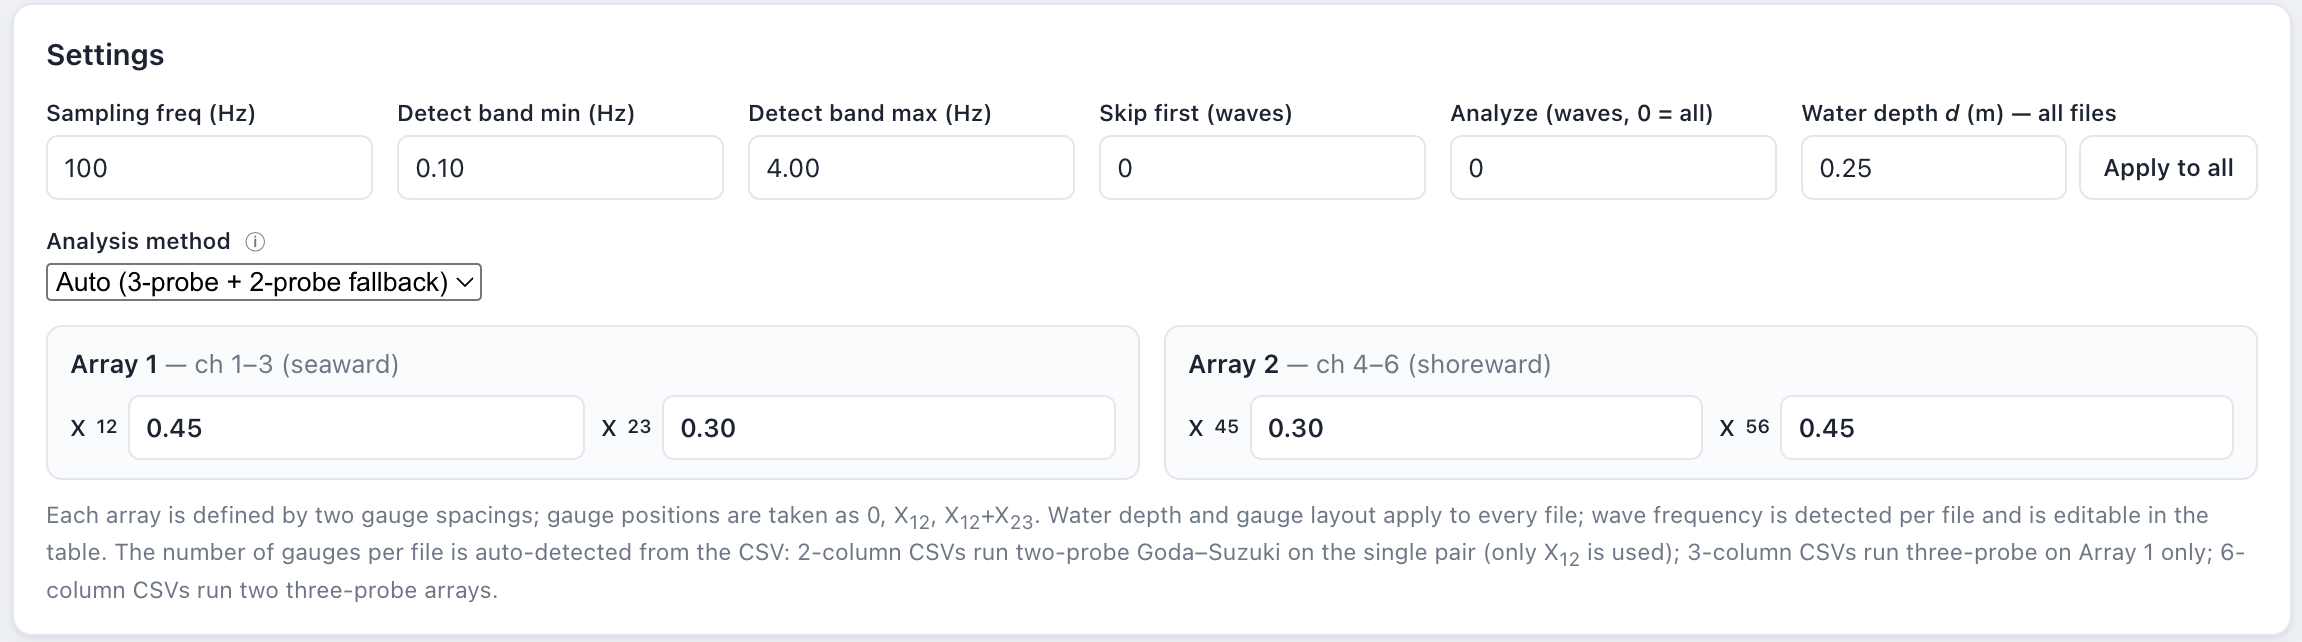
\includegraphics[width=17cm]{setting.png}};

% ===================== WORKFLOW STRIP (above) =============================
\node[stepbox, draw=wlxBlue,   fill=wlxBlueLt]   (w1) at (-6.6,4.35)
  {\textbf{1. Load}\\[1pt]{\footnotesize 6-channel CSV}};
\node[stepbox, draw=wlxViolet, fill=wlxVioletLt] (w2) at (-2.2,4.35)
  {\textbf{2. Configure}\\[1pt]{\footnotesize geometry \& depth}};
\node[stepbox, draw=wlxOrange, fill=wlxOrangeLt] (w3) at ( 2.2,4.35)
  {\textbf{3. Analyze}\\[1pt]{\footnotesize three-probe method}};
\node[stepbox, draw=wlxTeal,   fill=wlxTealLt]   (w4) at ( 6.6,4.35)
  {\textbf{4. Inspect}\\[1pt]{\footnotesize plots \& CSV export}};
\draw[warr] (w1.east) -- (w2.west);
\draw[warr] (w2.east) -- (w3.west);
\draw[warr] (w3.east) -- (w4.west);

% ===================== TITLE ==============================================
\node[font=\large\bfseries, text=wlxInk] at (0,5.95)
  {The WaveLabX Browser Application --- Client-Side Reflection Analysis};

% ===================== VISUALIZATION ROW (below settings) =================
\node[panel] (vts) at (-5.8,-4.35)
  {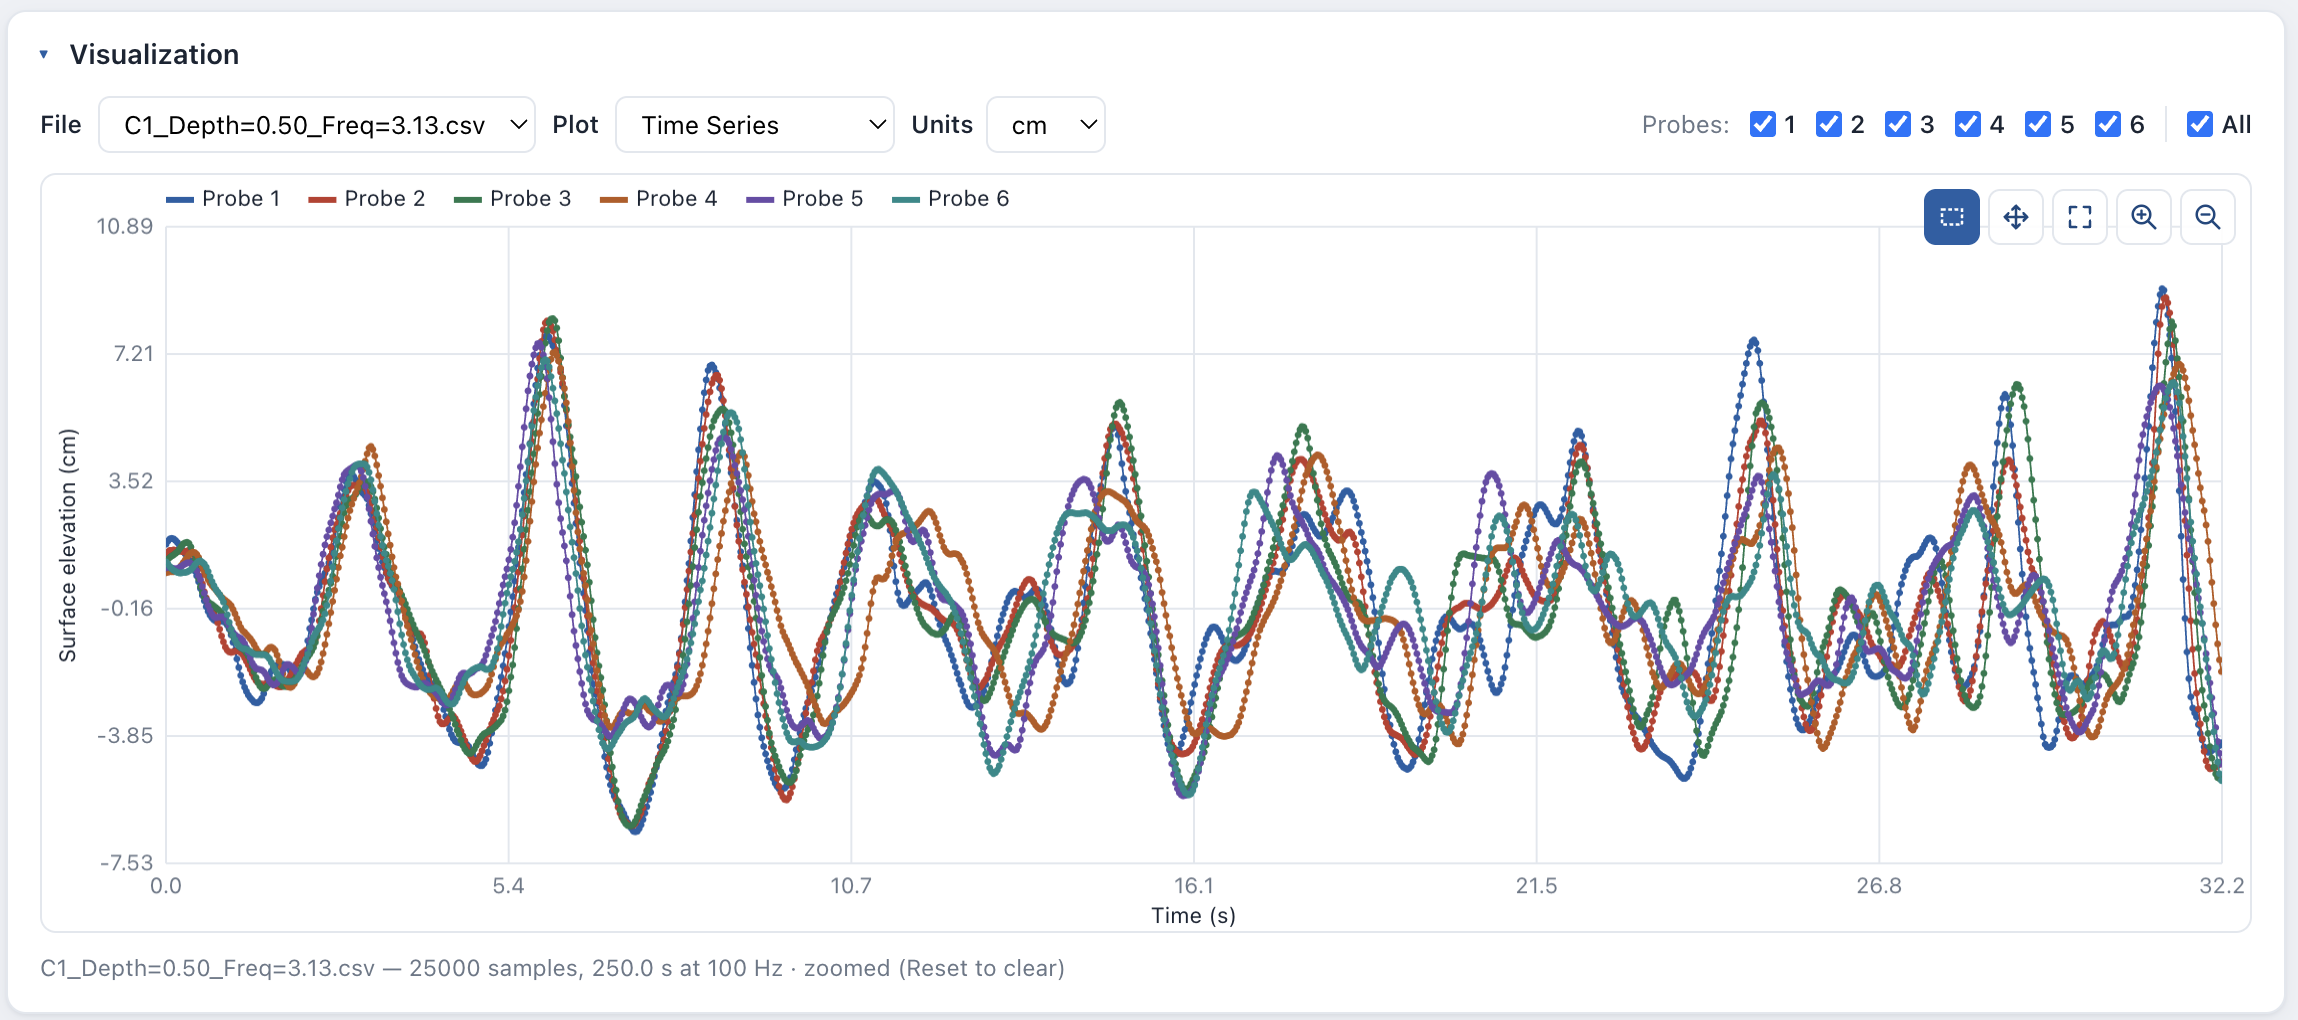
\includegraphics[width=5.4cm]{Visualization1.png}};
\node[panel] (ves) at ( 0.0,-4.35)
  {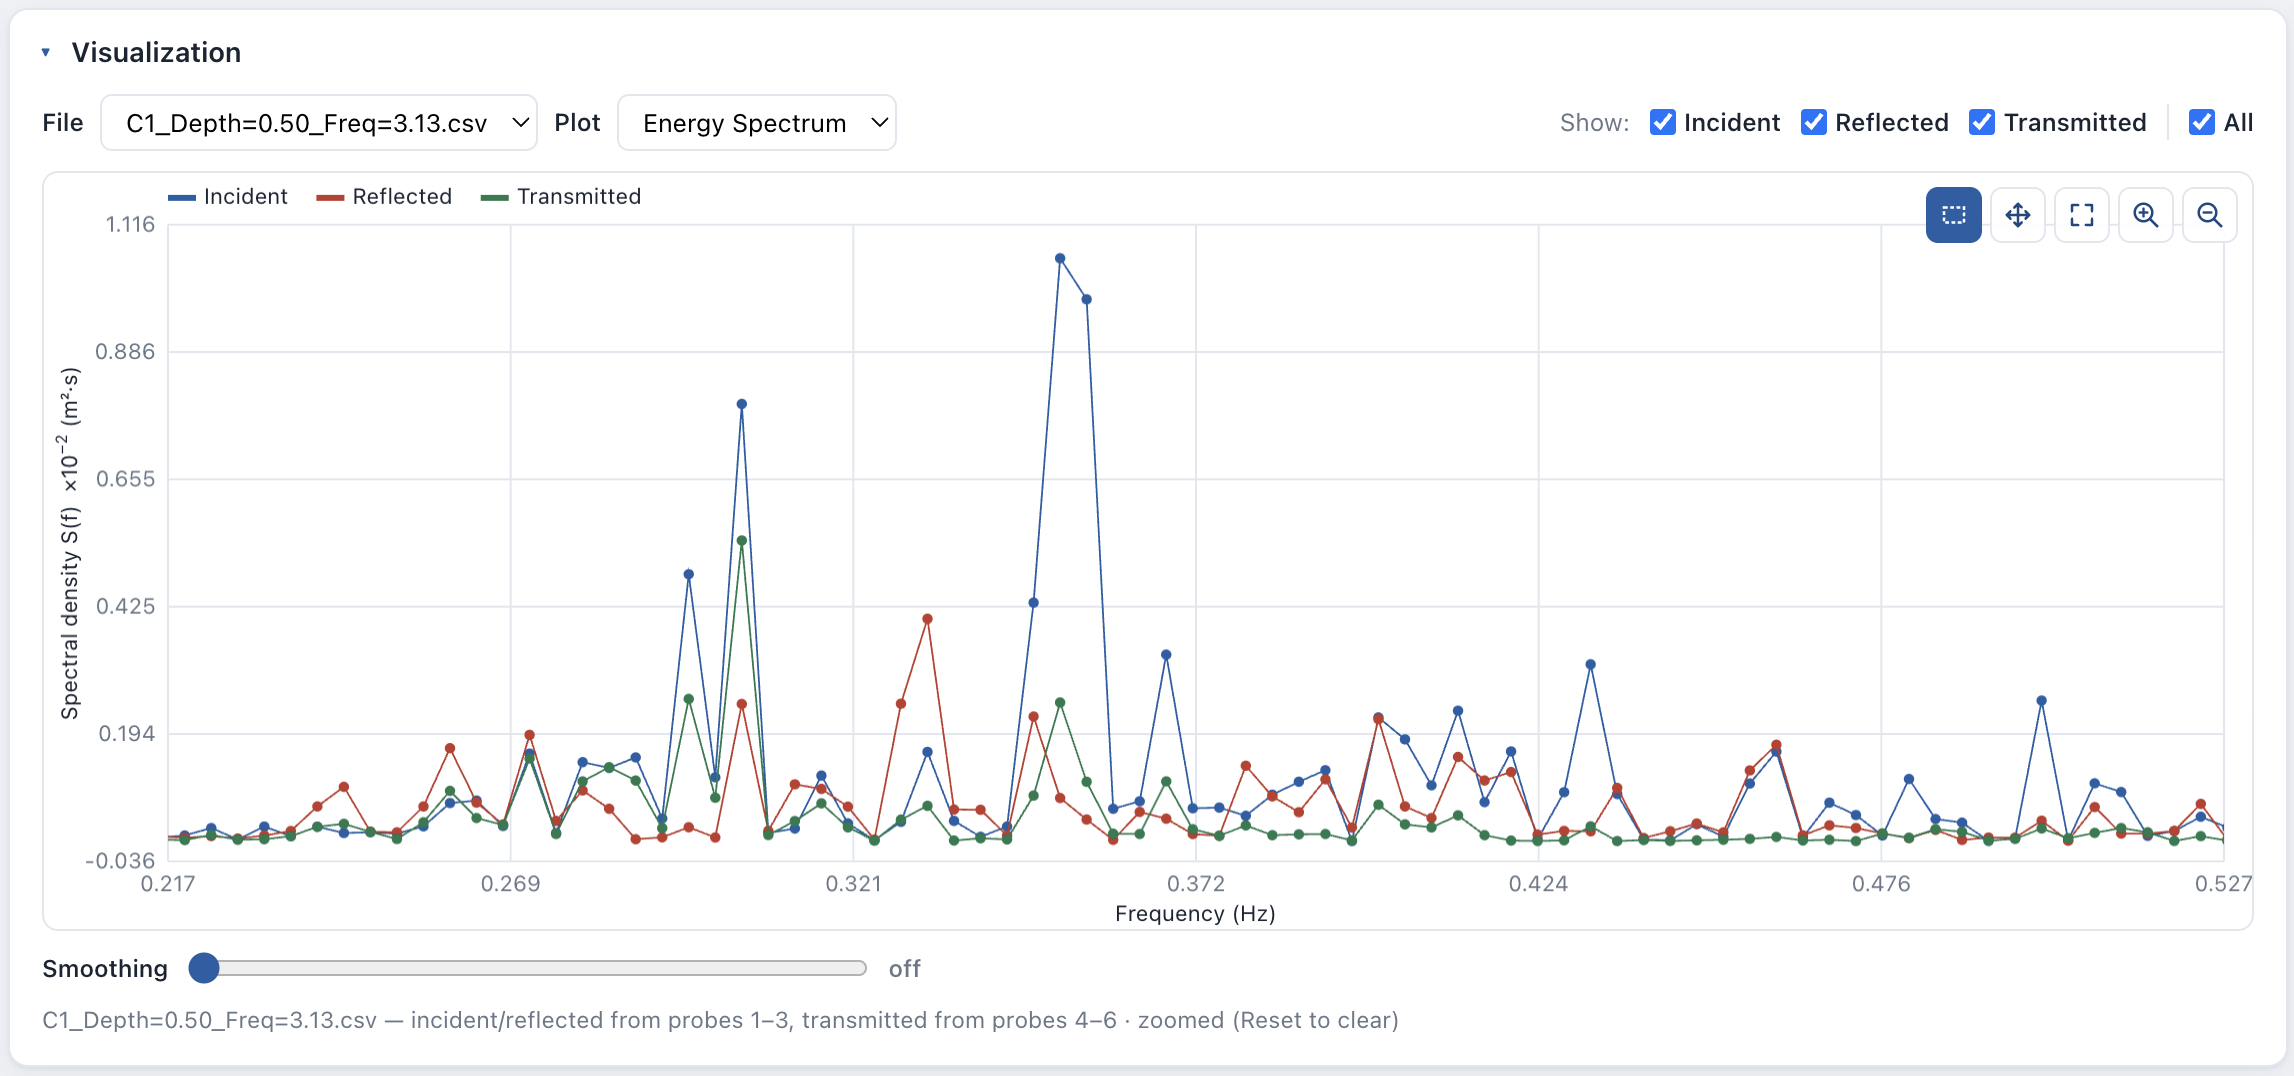
\includegraphics[width=5.4cm]{Visualization2.png}};
\node[panel] (vps) at ( 5.8,-4.35)
  {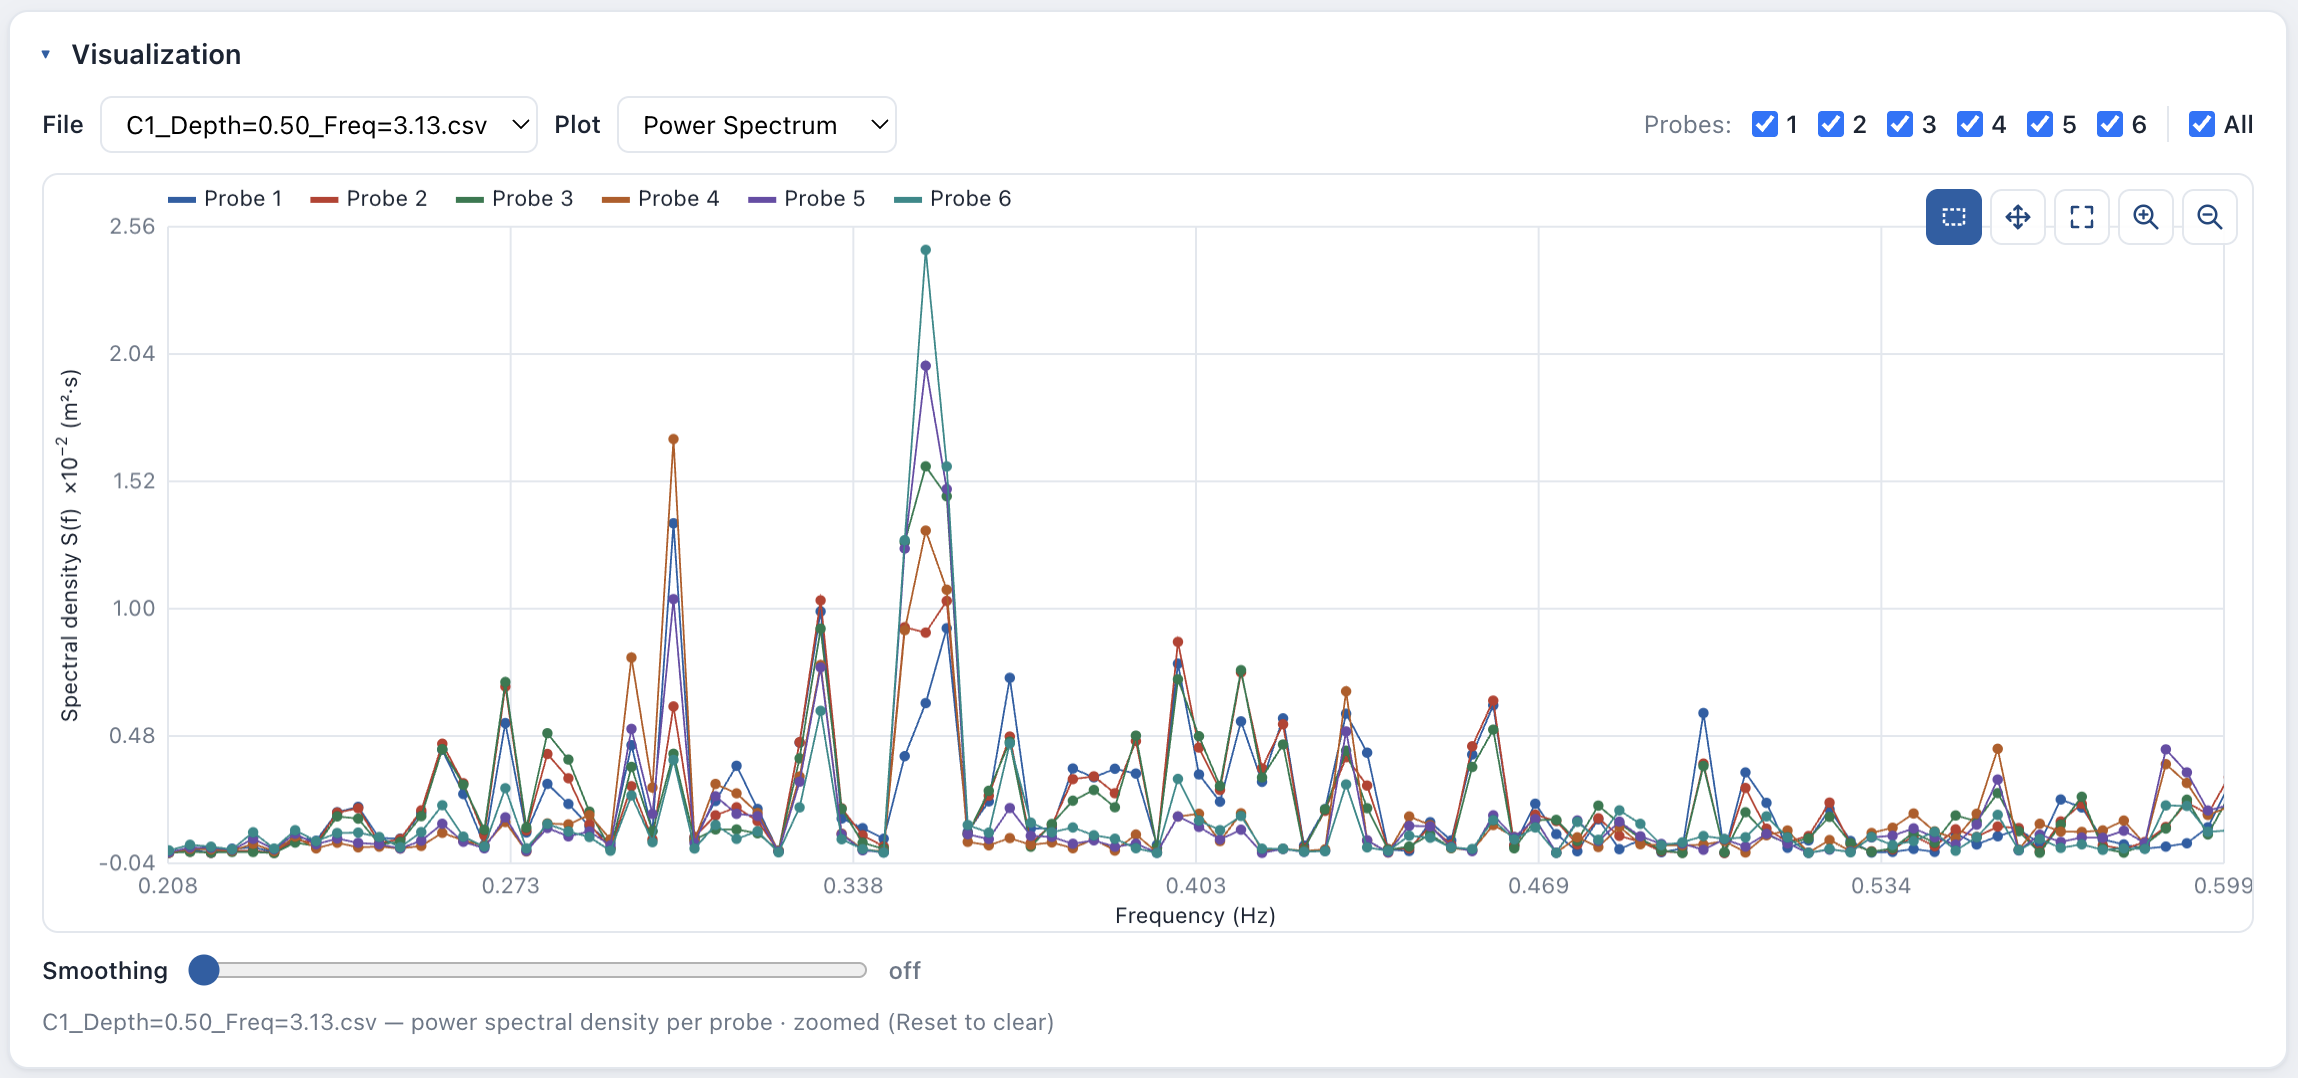
\includegraphics[width=5.4cm]{Visualization3.png}};

% ===================== RESULTS PANEL (bottom) =============================
\node[panel] (results) at (0,-7.30)
  {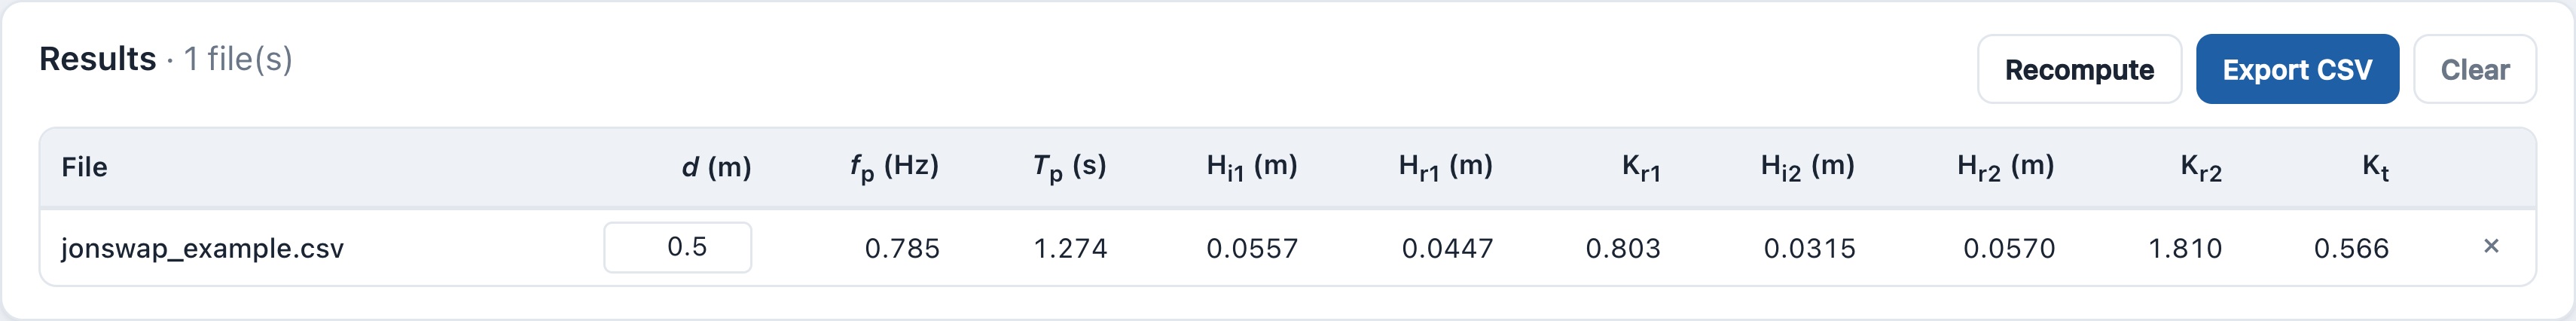
\includegraphics[width=17cm]{results.png}};

% ===================== PANEL LABELS =======================================
\node[plabel] at (-8.5,2.55)
  {(a)\quad Configuration: probe arrays, sampling rate and water depth};
\node[plabel] at (-8.5,-3.05) {(b)\quad Time series};
\node[plabel] at (-2.7,-3.05) {(c)\quad Energy spectrum};
\node[plabel] at ( 3.1,-3.05) {(d)\quad Power spectrum};
\node[plabel] at (-8.5,-6.05)
  {(e)\quad Per-file results: incident/reflected heights and coefficients};

\end{tikzpicture}
\end{document}
